%  PARA TRABALLOS EN GALLEGO USAR (LINEA 12): \usepackage[galician]{babel}
%  PARA TRABALLOS EN CASTELLANO USAR (LINEA 13): \usepackage[spanish]{babel}
%
% Para los acentos usamos codificacion UTF-8 (LINEA 10): \usepackage[utf8]{inputenc} 
% Si se usase la codificacion es_ES.ISO-8859-1 (LINEA 11): \usepackage[latin1]{inputenc}
% La conversion de acentos se hace con: iconv -f UTF-8 -t ISO-8859-1 filename.tex
%
% Como se incluyen figuras eps hay que compilar con: latex traballo , dvipdf traballo
%

\documentclass[12pt,twoside,a4paper]{book}
% pódense engadir todos os packages necesarios
\usepackage[utf8]{inputenc}
% \usepackage[latin1]{inputenc}
%\usepackage[galician]{babel}
\usepackage[spanish]{babel}
\usepackage{graphicx}
\usepackage[dvips]{epsfig}
\usepackage{amssymb}
\usepackage{eurosym}
\usepackage{float}
\usepackage{latexsym}
\usepackage{a4}
\usepackage{listings}
\usepackage{multirow}
\usepackage[hidelinks]{hyperref} % menús no pdf pero non leva ben co package galician
\usepackage{url}
\usepackage{rotating}
\usepackage{caption}
\usepackage[section]{placeins}
\usepackage{booktabs}
\usepackage{tabularx} % Better tables
\usepackage{enumitem}
\usepackage{xcolor}
\usepackage{xstring, xifthen}
\usepackage[nottoc, notlot, notlof, notindex]{tocbibind}

%%% Datos del TFG
\newcommand{\tfgauthor}{Rub{\'e}n Mosquera Varela}
\newcommand{\tfgtutor}{Jos{\'e} Ram{\'o}n R{\'i}os Viqueira}
\newcommand{\tfgcotutor}{Manuel Antonio Regueiro Seoane}
\newcommand{\tfgtitle}{Visualización de observacións en SIX de escritorio}
\newcommand{\tfgsubtitle}{}
\newcommand{\tfgtitleshort}{Visualización de observacións en SIX de escritorio} %Para meta-datos PDF
\newcommand{\tfgcopyright}{Copyright (C) 2015, \tfgauthor}
\newcommand{\tfglicense}{Creative Commons (by-sa) 2.5 Spain}
\newcommand{\tfglicenseurl}{http://creativecommons.org/licenses/by-sa/3.0/}
\newcommand{\tfgkeywords}{QGIS SOS OGC Observation}
\newcommand{\logoUni}{images/logo_usc.eps} % Logotipo de la Universidad

%%%
% CONFIG: Meta-datos para inclusión en PDF y XMP
%
\hypersetup{
    pdftitle        = {\tfgtitleshort},
    pdfauthor       = {\tfgauthor},
    pdfsubject      = {\tfgtitle},
    pdfkeywords     = {\tfgkeywords},
    pdfcreator      = {\tfgauthor},
    pdfproducer     = {\tfgauthor~powered~by~\LaTeX},
%    pdfcopyright    = {\tfgcopyright},
%    pdflicenseurl   = {\tfglicenseurl},
%    pdfstartview    = FitH % Ajustar la página a la ventana
}

%----------------------------------------------------------------------------------------
%	FLOATS: TABLES, FIGURES AND CAPTIONS SETUP
%----------------------------------------------------------------------------------------

%RISCOS
\newcounter{riskcnt}
\newcommand{\risktable}[7]{
	\renewcommand{\theriskcnt}{#1}
	\refstepcounter{riskcnt}
	~\\
	\noindent\colorbox{gray!20}{\parbox{\textwidth}{\hspace{0.4cm}\textsc{{#1}.- {#2}}}}\label{rsc:#1}
	\begin{description}[style=multiline,labelindent=0.4cm,leftmargin=4.7cm,itemsep=1pt, partopsep=10pt]
 	\item[Descrición] #3
 	\item[Probabilidade] #4 
 	\item[Impacto] #5 
 	\item[Nivel de exposición] #6 
 	\item[Resposta ao risco] #7 
	\end{description}
	%Se referencia con \ref{rsc:#1}.
	\addcontentsline{lot}{table}{{\theriskcnt} #2}
}
%CASOS DE USO
\newcounter{uccnt}
\newcommand{\uctable}[7]{
	\renewcommand{\theuccnt}{#1}
	\refstepcounter{uccnt}
	~\\
	\noindent\colorbox{gray!20}{\parbox{\textwidth}{\hspace{0.4cm}\textsc{{#1}.- {#2}}}}\label{uc:#1}
	\begin{description}[style=multiline,labelindent=0.4cm,leftmargin=4.5cm,itemsep=1pt, partopsep=10pt]
 	\item[Propósito] #3 
 	\item[Actores] Usuario
 	\item[Relacións] #4 
 	\item[Precondicións] #5 
 	\item[Poscondicións] #6
 	\item[Escenario] #7
	\end{description}
	%Se referencia con \ref{uc:#1}.
	\addcontentsline{lot}{table}{{\theuccnt} #2}
}

%REQUISITOS
\newcounter{reqcnt}
\newcommand{\reqtable}[5]{
	\renewcommand{\thereqcnt}{#1}
	\refstepcounter{reqcnt}
	~\\
	\noindent\colorbox{gray!20}{\parbox{\textwidth}{\hspace{0.4cm}\textsc{{#1}.- {#2}}}}\label{req:#1}
	\begin{description}[style=multiline,labelindent=0.4cm,leftmargin=4.5cm,itemsep=1pt, partopsep=10pt]
 	\item[Descrición] #3 
 	\item[Relevancia] #4
 	\item[Criterio de validación] #5 
	\end{description}
	%Se referencia con \ref{req:#1}.
	\addcontentsline{lot}{table}{{\thereqcnt} #2}
}

%PROBAS
\newcounter{testcnt}
\newcommand{\testtable}[5]{
	\renewcommand{\thetestcnt}{#1}
	\refstepcounter{testcnt}
	~\\
	\noindent\colorbox{gray!20}{\parbox{\textwidth}{\hspace{0.4cm}\textsc{{#1}.- {#2}}}}\label{test:#1}
	\begin{description}[style=multiline,labelindent=0.4cm,leftmargin=4.5cm,itemsep=1pt, partopsep=10pt]
 	\item[Requirimentos relacionados] #3 
 	\item[Descrición] #4
 	\item[Resultado] #5 
	\end{description}
	%Se referencia con \ref{test:#1}.
	\addcontentsline{lot}{table}{{\thetestcnt} #2}
}

%----------------------------------------------------------------------------------------
%	HYPHENATION
%----------------------------------------------------------------------------------------
\hyphenation{In-te-re-se}
\hyphenation{CiTIUS}
\hyphenation{unha}
\hyphenation{SOSClient}
\hyphenation{SOSClientDialog}
\hyphenation{SOSPlot}
\hyphenation{QgsMapToolCaptureSpatialOperand}
\hyphenation{SOSPlotDialog}
\hyphenation{GetObservations}
\hyphenation{GetCapabilities}
\hyphenation{Python}
%\includeonly{capitulos/titulo,capitulos/certificacion,capitulos/xestiondoproxecto}
%\includeonly{capitulos/analise}
\begin{document}
%%Se reeditan estas funciones para sacar el texto en gallego usando el idioma spanish, porque galician no funciona con hyperref
\renewcommand{\contentsname}{Índice xeral}
\renewcommand{\listtablename}{Índice de cadros}
\renewcommand{\tablename}{Cadro} 
\pagestyle{empty}
\begin{center}
{\bf\Large UNIVERSIDADE DE SANTIAGO DE COMPOSTELA}

\vspace{0.5cm}
\includegraphics[width=5cm]{\logoUni}

\vspace{0.5cm}
{\bf\large ESCOLA TÉCNICA SUPERIOR DE ENXEÑARÍA}

\vspace{2cm}
{\bf\LARGE \tfgtitle}

\vspace{0.5cm}
{\bf\LARGE \tfgsubtitle}
\end{center}

\vspace{2cm}
\hspace{4cm}\begin{tabular}{l}
{\it\Large Autor:} \\
{\bf\Large \tfgauthor} \\
~ \\
{\it\Large Directores:} \\
{\bf\Large \tfgtutor} \\
{\bf\Large \tfgcotutor} \\
\end{tabular}

\vspace{2cm}
\begin{center}
{\bf\Large Grao en Enxeñaría Informática}

\vspace{0.5cm}
{\bf\large Xullo 2015}

\vspace{0.5cm}
Traballo de Fin de Grao presentado na Escola Técnica Superior de Enxeñaría da Universidade de Santiago de Compostela para a obtención do Grao en Enxeñaría Informática
\end{center}


\cleardoublepage
\pagestyle{plain}
\pagenumbering{roman}
\includegraphics[width=4cm]{images/logo_usc.eps}

\vspace{1cm}
{\bf D. \tfgtutor}, Profesor do Departamento de Electrónica e Computación da Universidade de Santiago de Compostela, e {\bf D. \tfgcotutor}, TODO poñer aquó o cargo,

\vspace{1cm}
INFORMAN:

\vspace{1cm}
Que a presente memoria, titulada {\it \tfgtitle}, presentada por {\bf D. \tfgauthor} para superar os créditos correspondentes ao Traballo de Fin de Grao da titulación de Grao en Enxeñaría Informática, realizouse baixo nosa dirección no Departamento de Electrónica e Computación da Universidade de Santiago de Compostela.

\vspace{1cm}
E para que así conste aos efectos oportunos, expiden o presente informe en Santiago de Compostela, a 10 de Xullo de 2015:

\vspace{2cm}
\begin{tabular}{lll}
O titor, & O cotitor, & O alumno, \\
~ \\
~ \\
~ \\
~ \\
~ \\
~ \\
~ \\
\tfgtutor & \tfgcotutor & \tfgauthor
\end{tabular}

 % paxina de certificación (optativa)
%\cleardoublepage
%\pagestyle{plain}
\chapter*{Agradecementos}
A Olatz, pola motivación, o ánimo e o apoio. % paxina de agradecementos (optativa) 
\cleardoublepage
\pagestyle{plain}
\chapter*{Resumo}
TODO

 % páxina de resumo (optativa) 

\cleardoublepage
\pagestyle{plain}
\tableofcontents
\listoffigures
\listoftables

% Agora incluimos os capítulos. Cambiamos a numeración e as cabeceiras
\cleardoublepage
\pagenumbering{arabic}
\setcounter{page}{1}
\pagestyle{headings}
\chapter{Introdución}
a)Introdución:  composta  por  Obxectivos  Xerais,  Relación  da  Documentación  que  conforma  a 
Memoria,  Descrición  do  Sistema,  Información  Adicional  de  Interese  (métodos,  técnicas  ou 
arquitecturas utilizadas, xustificación da súa elección, etc.). 
 
\section{Contextualización}
\section{Motivación e Obxectivos}
\section{Estrutura da memoria}

Este documento estrutúrase en 6 capítulos, dous apéndices e a bibliografía empregada.

\begin{description}
\item[Capítulo 1:] \textit{Introdución.}
\item[Capítulo 2:] \textit{Xestión do proxecto.} Neste capítulo abórdanse os aspectos relativos á xestión do proxecto: a definición do alcance, a metodoloxía, planificación temporal e xestión de riscos e da configuración.
\item[Capítulo 3:] \textit{Análise de requisitos.}
\item[Capítulo 4:] \textit{Deseño de software.}
\item[Capítulo 5:] \textit{Implementación e probas.}
\item[Capítulo 6:] \textit{Conclusións e traballo futuro.}
\item[Apéndice A:] \textit{Manual técnico.}
\item[Apéndice B:] \textit{Manual de usuario.}
\item[Bibliografía:] Referencias consultadas para o desenvolvemento do proxecto.
\end{description}
\cleardoublepage
\chapter{Xestión do proxecto}
A xestión do proxecto ten como finalidade definir e alcanzar os obxectivos do mesmo, ó tempo que se optimiza o uso de recursos, tanto humanos como materiais. Na sección III do PMBOK\cite{PMBOK} descríbense amplamente os distintos tipos de procesos que se inclúen dentro da xestión do proxecto, non obstante, para cada proxecto concreto será necesario seleccionar os máis apropiados para cumprir co obxectivo do mesmo.

\section{Alcance do proxecto}
Os procesos de xestión do alcance do proxecto son os encargados de asegurar que o proxecto inclúa o traballo requirido, e só o requirido, para completar o proxecto de forma satisfactoria.

\subsection{Definición do alcance}
O obxectivo deste proxecto é dotar ó Sistema de Información Xeográfica QGIS\footnote{http://www.qgis.org/} da capacidade de consultar fontes de datos SOS e representar os datos obtidos no contorno de mapas proporcionado pola ferramenta, de xeito que podan ser explorados e analizados polo usuario. Para acadar este obxectivo desenvolverase un engadido para o programa QGIS, coas seguintes funcionalidades:

\begin{itemize}
\item Conectarse a un servidor SOS e obter as capacidades do servizo a través da operación GetCapabilities.
\item En base as capacidades do servidor permitir xerar unha petición de observacións, de forma sinxela, sin necesidade de coñecementos técnicos do SOS.
\item Permitir modificar a petición xerada manualmente se o usuario o desexa.
\item Obter as observacións a través da operación GetObservations.
\item Coas observacións descargadas xerar unha capa vectorial que conteña a información xeográfica, temporal e os valores das propiedades observadas.
\item Xerar gráficos en dúas dimensións cos datos da capa.
\item Permitir visualizar a capa co plugin TimeManager de xeito que se podan facer animacións.
\end{itemize}

\subsection{Estrutura de Descomposición do Traballo}
A Estrutura de Descomposición do Traballo (EDT) axuda a dividir o proxecto en paquetes de traballo de forma xerárquica. Dado que se empregará a metodoloxía áxil \emph{Scrum} non é necesario detallar o EDT máis do que xa se fixo no anteproxecto, que se representa na figura \ref{fig:edt}.

\begin{figure}[hbtp]
\centering
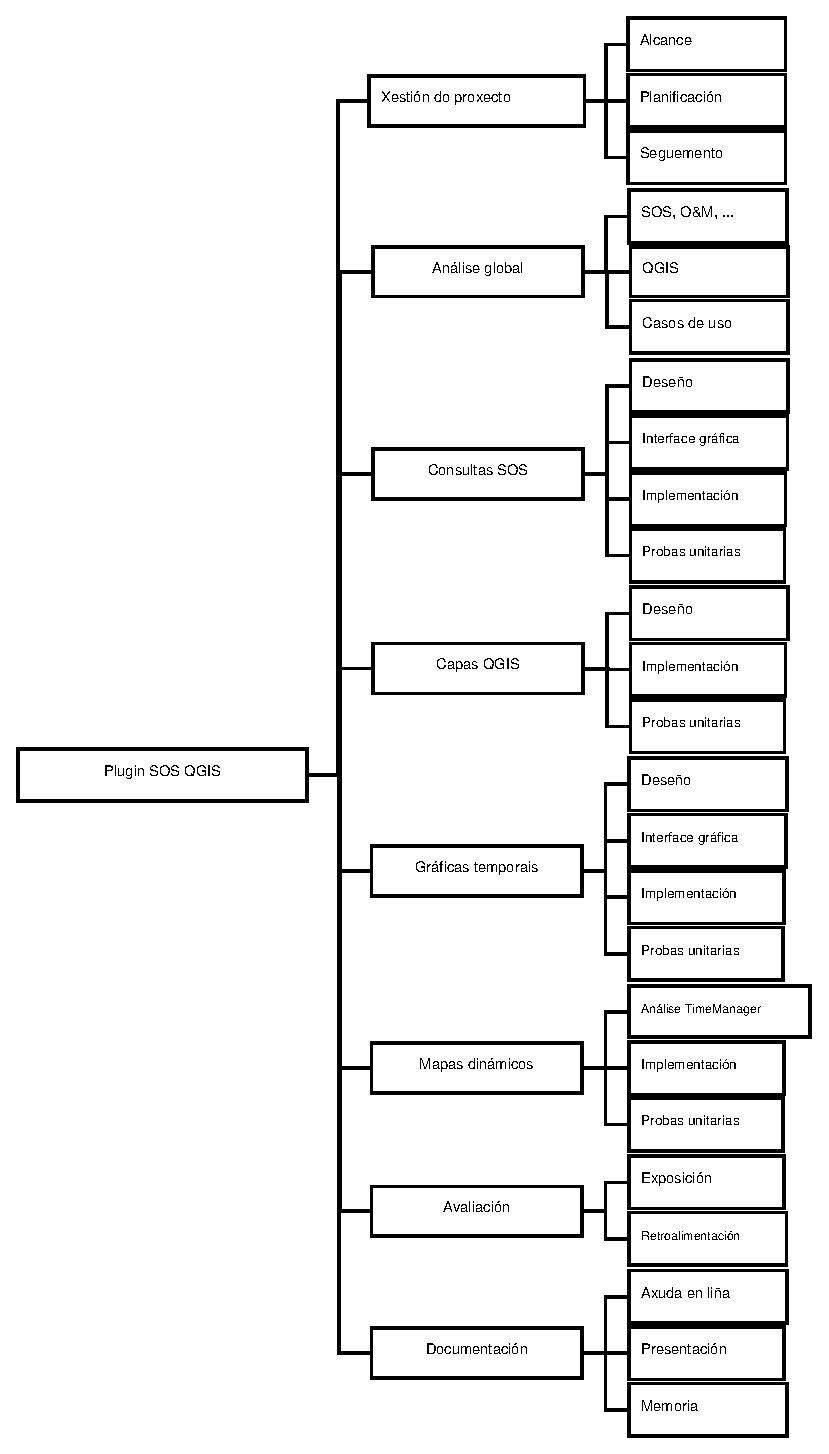
\includegraphics[scale=1]{images/edt.eps}
\caption{Estrutura de Descomposición do Traballo}
\label{fig:edt} 
\end{figure}

\section{Xestión do tempo}
A xestión do tempo do proxecto inclúe os procesos necesarios para lograr a conclusión do proxecto a tempo.

Ó empregar a metodoloxía \emph{Scrum} non se planifica inicialmente a duración de cada tarefa, non obstante si se poden identificar as distintas tarefas a levar a cabo e facer unha estimación da súa duración en base ás horas establecidas para o proxecto e a importancia de dita tarefa para a consecución dos obxectivos do proxecto. Así pois, o diagrama de Gantt da figura \ref{fig:gantt} debe interpretarse como unha estimación das horas a adicar a cada actividade e non como unha organización cronolóxica das actividades a realizar e fitos a acadar.

A continuación enuméranse as fases do EDT \ref{fig:edt} de máis alto nivel describindo a natureza das tarefas que inclúe cada unha delas e que se detallan no diagrama de Gantt \ref{fig:gantt}.

\section{Xestión do custo}
Debido a que este proxecto é un Traballo de Fin de Grao os custos manexados son teóricos e non se considerarán os custos indirectos (electricidade, internet e similares) ou gastos de desprazamento. A xestión de custos faise co único obxectivo de dar unha valoración económica realista do traballo realizado polo que se contemplarán os recursos humanos, os recursos materiais e os recursos software necesarios para a execución do proxecto.

\subsection{Custo de recursos humanos}
O equipo de desenvolvemento para a realización do proxecto consta dunha soa persoa, que realizará as distintas tarefas de análise, programación e documentación do mesmo. Os dous titores do proxecto non se consideran parte do equipo ó nivel de xestión de custos pois a este efecto actúan no rol de clientes.

Consideraremos como salario bruto anual para o recurso 24.000 \euro, que é segundo tecnoempleo.com\cite{InformeSalarios} o salario bruto medio para un analista/programador. Ó salario bruto débense engadir os custos do mesmo para a empresa, que tomando como referencia os datos da Seguridade Social\cite{TabCotizacion} suporía un 29,9\% do mesmo. Para o cálculo do custo por hora considerase a xornada máxima indicada no Convenio Colectivo\cite{BOEConvenio}, que son 1.800 horas de traballo ó ano.

O custo de recursos humanos é por tanto de 17,32 \euro/hora.

\subsection{Custo de recursos materiais}
Para o desenvolvemento do proxecto é necesario un ordenador capaz de executar QGIS. QGIS non especifica formalmente uns requirimentos mínimos e é capaz de funcionar de xeito fluído nun ordenador estándar que se pode adquirir por uns 600 \euro. Considerando unha porcentaxe de amortización anual do 25\%, como indica a Lei 27/2014\cite{Lei27/14}, pódense imputar como custes 12,50 \euro/mes. A estes efectos deben computarse os meses naturais de duración do proxecto.

Os materiais funxibles necesarios para a realización do proxecto e os gastos de impresión e CDs para a presentación do mesmo supoñen un custe de 140 \euro.

\subsection{Custo de recursos software}
Todas as ferramentas software empregadas para a realización deste proxecto son de uso gratuíto.

\subsection{Presuposto}
Na táboa \ref{tab:presuposto} amosase o resumo dos custos do proxecto, que suman un total de \euro.
\begin{table}[H]
\centering
\begin{tabularx}{\textwidth}{Xrrr} \toprule
	Concepto & Cantidade & Custo unitario & Total \\
	\midrule
	Custos de persoal & 420 horas & 17,32 \euro & 7274,40 \euro \\
	Amortización do ordenador & 6 meses & 12,50 \euro & 75,00 \euro \\
	Custos doutros materiais & 1 & 140,00 \euro & 140,00 \euro \\
	\midrule
	\multicolumn{3}{r}{\textbf{Total}} & \textbf{7489,40 \euro} \\
	\bottomrule
\end{tabularx}
\caption{Custos totais}
\label{tab:presuposto}
\end{table}

\section{Xestión de riscos}
A xestión de riscos ten como finalidade aumentar a probabilidade e o impacto de eventos positivos e diminuír a probabilidade e impacto dos eventos adversos para o proxecto. Implica, polo tanto, prever e xestionar os eventos que poden influír na planificación temporal, no esforzo ou no custo do proxecto ou na calidade do produto e tomar as accións necesarias para evitalos ou minimizar o seu impacto. Os catro pasos básicos a seguir para levar a cabo a xestión de riscos son:
\begin{itemize}
\item Identificación
\item Análise e catalogación
\item Planificación da resposta
\item Seguimento e control
\end{itemize}

Para catalogar os riscos en base a súa relevancia empréganse tres medidores: a probabilidade de que ocorra, o impacto que supón sobre o tempo ou esforzo, e o nivel de exposición, que é unha combinación dos valores de probabilidade e impacto. Os distintos valores para estes medidores recóllense na táboa \ref{tab:exposicion}

\begin{table}[H]
\centering
\begin{tabular}{@{}ccccc@{}}
\cmidrule(l){3-5}
\multicolumn{2}{c}{\multirow{2}{*}{}}                                                                       & \multicolumn{3}{c}{Probabilidade}                                                                                                                                                                                    \\ \cmidrule(l){3-5} 
\multicolumn{2}{c}{}                                                                                        & \begin{tabular}[c]{@{}c@{}}Case seguro\\ $\geq$80\%\end{tabular} & \begin{tabular}[c]{@{}c@{}}Moi probable\\ \textless80\% e \textgreater30\%\end{tabular} & \begin{tabular}[c]{@{}c@{}}Pouco probable\\ $\leq$30\%\end{tabular} \\ \midrule
\multirow{6}{*}{\rotatebox{90}{Impacto}} & \begin{tabular}[c]{@{}c@{}}Alto\\ $\geq$20\%\end{tabular}                & Alto                                                             & Alto                                                                             & Medio                                                          \\
                         & \begin{tabular}[c]{@{}c@{}}Medio\\ \textless20\% e \textgreater10\%\end{tabular} & Alto                                                             & Medio                                                                            & Baixo                                                          \\
                         & \begin{tabular}[c]{@{}c@{}}Baixo\\ $\leq$10\%\end{tabular}                   & Medio                                                            & Baixo                                                                            & Baixo                                                          \\ \bottomrule
\end{tabular}
\caption{Nivel de exposición dun risco en base a Probabilidade e Impacto}
\label{tab:exposicion}
\end{table}

\subsection{Especificación de riscos}
Co obxectivo de non engadir complexidade ó seguimento do proxecto so se planifican os riscos adversos con un nivel de exposición alto, é dicir, os riscos que é bastante probable que ocorran e que teñen un impacto negativo considerable sobre o desenvolvemento do proxecto. Para desenvolver respostas efectivas ós riscos é de moita utilidade agrupalos por causas comúns, neste caso clasificándoo en base á fonte do risco.

\subsubsection{Riscos técnicos}
\risktable	{R.TEC.01}{Complexidade do estándar SOS} %Id, Nome
			 %Descrición
		  	{O nivel de madurez e uso do estándar SOS fai que sexa un estándar extremadamente amplo e con un alto grao de liberdade. Non existe ningunha implementación que cubra o estándar na súa totalidade.}
			{Moi probable} %Probabilidade
			{Alto} %Impacto
			{Alto} %Nivel de exposición
			%Resposta
			{Só se comprometerá como imprescindible soportar as operacións básicas para obter os datos de observacións provistos pola implementación SOS realizada polo CiTIUS.}

\risktable	{R.TEC.02}{Escaseza de servidores SOS} %Id, Nome
			 %Descrición
		  	{Existen moi poucos servidores que implementen SOS abertos ó público cos que poder validar a implementación realizada.}
			{Case seguro} %Probabilidade
			{Medio} %Impacto
			{Alto} %Nivel de exposición
			%Resposta
			{Instalar en local un servidor SOS para poder probar a aplicación, e solicitar acceso ós xestionados polo CiTIUS.}
			
\subsubsection{Riscos externos}
\risktable	{R.EXT.01}{Soporte de SOS en QGIS} %Id, Nome
			 %Descrición
		  	{Implementación nativa dentro do QGIS do soporte para SOS ou a publicación de algún plugin que implemente dito soporte.}
			{Moi probable} %Probabilidade
			{Alto} %Impacto
			{Alto} %Nivel de exposición
			%Resposta
			{Reorientar o proxecto para centralo en dotar o QGIS de ferramentas específicas para interacción cos datos de sensores, sempre e cando a solución SOS implantada de soporte a implementación realizada polo CiTIUS.}

\subsubsection{Riscos de persoal}
\risktable	{R.PER.01}{Descoñecemento da ferramenta QGIS} %Id, Nome
			 %Descrición
		  	{O equipo de desenvolvemento non ten experiencia no manexo da ferramenta QGIS nin outras ferramentas de información xeográfica.}
			{Case seguro} %Probabilidade
			{Medio} %Impacto
			{Alto} %Nivel de exposición
			%Resposta
			{No plan de traballo do proxecto inclúese capacitación na ferramenta QGIS así como nos conceptos básicos sobre sistemas de información xeográfica.}

\risktable	{R.PER.02}{Descoñecemento da linguaxe Python} %Id, Nome
			 %Descrición
		  	{O equipo de desenvolvemento non ten experiencia na linguaxe de programación Python.}
			{Case seguro} %Probabilidade
			{Alto} %Impacto
			{Alto} %Nivel de exposición
			%Resposta
			{No plan de traballo do proxecto inclúese capacitación na linguaxe de programación Python PyQt4.}
			
\risktable	{R.PER.03}{Situación persoal dos membros do equipo} %Id, Nome
			 %Descrición
		  	{Cambios na situación persoal ou laboral nos membros do equipo que impidan levar a cabo a dedicación estimada.}
			{Case seguro} %Probabilidade
			{Alto} %Impacto
			{Alto} %Nivel de exposición
			%Resposta
			{Volver a planificar os prazos de execución do proxecto.}
			
\subsubsection{Riscos na xestión do proxecto}
\risktable	{R.XES.01}{Error na estimación temporal} %Id, Nome
			 %Descrición
		  	{A estimación temporal inicial para a execución das tarefas é pouco precisa a causa da inexperiencia en proxectos similares.}
			{Case seguro} %Probabilidade
			{Medio} %Impacto
			{Alto} %Nivel de exposición
			%Resposta
			{A estimación inicial realizase de forma pesimista. A metodoloxía \emph{Scrum} minimiza o impacto ó permitir a refinación de requisitos e estimacións o longo do proxecto.}

\section{Xestión da configuración}
A xestión da configuración \cite{GPGC} ten como propósito establecer e manter a integridade dos elementos de traballo. No proxecto que nos ocupa os elementos de traballo a xestionar son o código fonte do \emph{plugin}, o código fonte da documentación, e os distintos entregables xerados.

\subsection{Control do código fonte}
Dentro do código fonte a xestionar inclúese tanto o código do aplicación, imaxes, documentos de axuda e demais que si inclúen no \emph{plugin} empaquetado, como o código fonte para xerar a documentación.

En ambos casos o procedemento de xestión da configuración se fai a través do sistema de xestión de versións \emph{Git}. Mantéñense en local dous repositorios diferentes, un para aplicación e outro para documentación, cada un coa súa réplica remota correspondente aloxada en \emph{GitHub}\footnote{https://github.com/}. As carpetas dos repositorios locais replícanse en Dropbox\footnote{https://www.dropbox.com/} co obxectivo de ter unha copia redundante na nube e acceso desde distintos ordenadores en todo momento.

O método de traballo consiste en realizar un \emph{Commit} local cada vez que se remata unha tarefa e realizar un \emph{Push} ó servidor remoto cada vez que se remata unha versión susceptible de ser publicada. Deste xeito no repositorio público sempre hai unha versión estable do produto.

\subsection{Control dos entregables}
Os distintos obxectos entregables xerados o longo do proxecto, dende o anteproxecto ata a presentación do mesmo son arquivados tanto en local como na carpeta de Dropbox. Non se realiza máis control de versións sobre os produtos entregables que o propio control realizado por Dropbox. Esta ferramenta permite o acceso ás distintas versións gardadas de calquera tipo de ficheiro.

O servizo Dropbox tamén permite a creación de carpetas públicas. Esta funcionalidade permítenos crear un repositorio público para QGIS no que aloxar o \emph{plugin} empaquetado de xeito que sexa moi sinxelo de instalar.\cleardoublepage
\chapter{Análise de requisitos}

A análise dos requisitos dun produto software é unha parte fundamental do proceso de desenvolvemento, pois consiste definir de forma detallada o que debe facer o produto para satisfacer as necesidades e cumprir as expectativas do cliente.

O proceso de xestión de requisitos\cite{GPGR} consistirá en definir conxuntamente co cliente os distintos casos de uso do software. A partir dos casos de uso identificados extráense e documéntanse os requisitos, que se usarán como referencia para o desenvolvemento do sistema.

\section{Casos de uso}

Os casos de uso\cite{UseCase} describen as interaccións entre os actores é o sistema nunha linguaxe non técnica, centrándose en que fai o sistema para o actor, entendendo por actor calquera entidade externa ó sistema que lle demande algunha funcionalidade.

Neste proxecto identifícase un único actor, que é o usuario xenérico da aplicación, pois nin existen distintos roles de usuarios nin outras entidades externas.

A continuación descríbense os casos de uso identificados en colaboración cos directores do proxecto, que exercen o rol de cliente, e que se resumen graficamente na figura \ref{fig:uc}.

\uctable 	{CU.01}{Consultar as capacidades dun servidor SOS}
			{Consultar as capacidades dun servidor SOS para ver as ofertas que realiza e as propiedades dispoñibles nelas, e demais información do servizo.} %Propósito
			{É estendido polo \ref{uc:CU.02}} %Relacións
			{-} %Precondicións 
			{Visualízanse as capacidades do SOS nun formato amigable para o usuario.} %Postcondicións
			{O usuario introduce o enderezo do servidor SOS, ou selecciónao de entre os gardados. A aplicación descarga as capacidades do mesmo para amosalas en pantalla. 
			} %Escenario
			
\uctable 	{CU.02}{Obter observacións do servidor SOS}
			{Xerar unha capa vectorial cos datos das observacións rexistradas no SOS.} %Propósito
			{Estende o \ref{uc:CU.01}} %Relacións
			{Ter consultado as capacidades do servizo.} %Precondicións 
			{Capa vectorial coas observacións obtidas.} %Postcondicións
			{O usuario selecciona a través da interface gráfica a oferta e propiedades a consultar, así como outros filtros máis avanzados, por entidade de interese, sensor, período de tempo, filtros espaciais, etc. A aplicación descarga as observacións e xera unha capa vectorial en QGIS coa información procesada.
			} %Escenario

\uctable 	{CU.03}{Visualizar gráficas en dúas dimensións}
			{Visualizar nunha gráfica en dúas dimensións a información das observacións, a partir da capa xerada. Débese poder visualizar a evolución dunha propiedade con respecto ó tempo, e tamén sería de utilidade en algúns caso poder enfrontar unha propiedade contra outra. } %Propósito
			{-} %Relacións
			{Ter xerada unha capa con datos de observacións.} %Precondicións 
			{Gráfico en dúas dimensións dos datos seleccionados.} %Postcondicións
			{Sobre a capa xerada o usuario seleccionará entidades de interese para poder visualizar nunha nova ventá un gráfico que represente o tempo no eixo X e a propiedade indicada no eixo Y. O usuario pode seleccionar outra propiedade para representar en cada un dos eixos.
			} %Escenario
			
\uctable 	{CU.04}{Visualizar mapas animados}
			{Facer visualizacións animadas dos datos da capa dentro do propio visor de mapas de QGIS.} %Propósito
			{-} %Relacións
			{Ter xerada unha capa con datos de observacións.} %Precondicións 
			{Visualización animada das observacións.} %Postcondicións
			{O usuario disporá duns controis de reprodución para as capas con datos de observacións de xeito que poda reproducir a evolución cronolóxica das observacións sobre o propio visor de mapas de QGIS. 
			} %Escenario

\begin{figure}[hbtp]
\centering
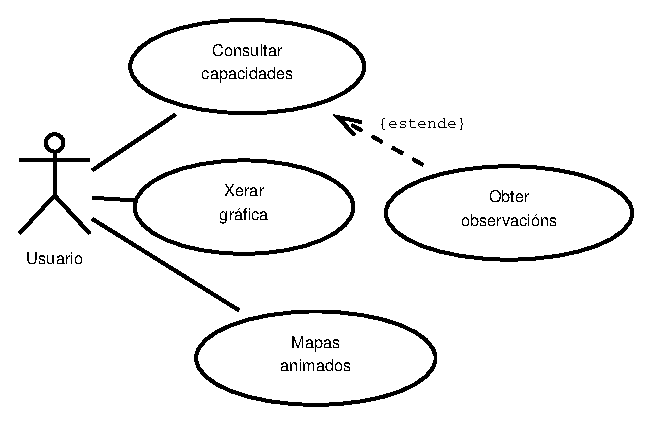
\includegraphics[width=0.8\textwidth]{images/uc.eps}
\caption{Diagrama de casos de uso}
\label{fig:uc} 
\end{figure}

\section{Catálogo de requisitos}
A partir dos casos de uso documentados realizase a extracción dos requisitos da aplicación. Estes requisitos son as características que debe presentar a aplicación, e definen o software desde o punto de vista do cliente. Dividimos os catálogo de requisitos en dúas partes, segundo a natureza dos mesmos:
\begin{description}
\item[Funcionais:] Son as características da aplicación para proporcionar a funcionalidade requirida.
\item[Non funcionais:] Non describen funcionalidades, se non que representan outras necesidades como seguridade, rendemento, usabilidade, ou restricións de plataforma, tecnolóxicas, e similares.
\end{description}

Clasificaremos os requisitos pola súa relevancia segundo o cadro \ref{tab:relevanciaReq}, que se terá en conta na planificación dos sprints.
\begin{table}
\begin{tabularx}{\textwidth}{lX} \toprule
	Relevancia & Descrición \\
	\midrule
	Esixido & Requisito que está directamente relacionado co cumprimento dos obxectivos do proxecto.\\
	Desexado & Requisito que mellora a calidade do proxecto, pero non está relacionado directamente cos obxectivos do mesmo.\\
	Opcional &  Requisito que non supón unha mellora substancial na calidade do proxecto, aínda que si resulta de utilidade.\\
	\bottomrule
\end{tabularx}
\caption{Niveis de relevancia dun requisito}
\label{tab:relevanciaReq}
\end{table}

\subsection{Requisitos funcionais}
Os requisitos funcionais definidos, verificados e revisados para o presente proxecto son os que seguen:

\reqtable 	{RF.01}{Conectar con servidor SOS}
		  	{O usuario pode introducir o enderezo dun servidor que proporcione o servizo SOS e obter do mesmo as súas capacidades. Estas capacidades deben visualizarse nun formato amigable para o usuario.}%Descrición
			{Esixido}%Relevancia
			{O requisito cumprirase se a aplicación e capaz de conectarse cos servidores indicados e procesar o resultado da operación \emph{GetCapabilities} para visualizala nun formato lexible.}%Criterio de validación
			
\reqtable 	{RF.02}{Gardar lista de servidores SOS}
		  	{O usuario poderá xestionar unha lista de servidores SOS para os que se indicará o enderezo e un nome para identificalo.}%Descrición
			{Opcional}%Relevancia
			{O requisito cumprirase se a aplicación permite gardar unha lista de servidores e facer o mantemento da mesma.}%Criterio de validación
			
\reqtable 	{RF.03}{Visualizar XML das capacidades do servidor}
		  	{O usuario poderá visualizar en formato texto, con resaltado de sintaxe, e nun visor de árbore o XML que describe as capacidades do servidor.}%Descrición
			{Desexado}%Relevancia
			{O requisito cumprirase se a aplicación dispón dun visor de XML con resaltado de sintaxe e visor de árbore no que se amose o ficheiro resposta do servidor á petición \emph{GetCapabilities}.}%Criterio de validación
			
\reqtable 	{RF.04}{Xerar capa vectorial cas observacións do servidor}
		  	{Unha vez consultadas as capacidades do servidor, o usuario poderá seleccionar unha oferta e unha ou varias das propiedades da mesma para descargar os datos e xerar unha capa vectorial coas observacións descargadas.}%Descrición
			{Esixido}%Relevancia
			{O requisito cumprirase se a aplicación descarga os datos solicitados do servidor e procesa o XML para crear un rexistro na capa vectorial para cada observación, cos datos de xeometría, tempo e o valor de cada propiedade.}%Criterio de validación

\reqtable 	{RF.05}{Permitir filtrado básico das observacións a descargar}
		  	{O usuario poderá indicar o rango de tempo do que lle interesan as observacións, así como un ou máis sensores e unha ou máis entidades.}%Descrición
			{Esixido}%Relevancia
			{O requisito cumprirase se a través de interface se pode seleccionar un rango de tempo, unha lista de sensores e unha lista de entidades e estes datos se inclúen no XML para a operación \emph{GetObservations}.}%Criterio de validación
\newpage			
\reqtable 	{RF.06}{Permitir filtrado avanzado das observacións a descargar}
		  	{O usuario poderá indicar un filtro espacial que delimite a zona da que quere obter as observacións. A interface mostrará os operadores e tipos de operandos soportados polo servizo. Tamén se poderá indicar un filtro escalar por algunha das propiedades da oferta seleccionada. A interface so mostrará os operandos soportados polo servizo.}%Descrición
			{Desexado}%Relevancia
			{O requisito cumprirase se a través de interface se pode indicar un filtro espacial, seleccionando a xeometría sobre o mapa, e un filtro escalar para algunha das propiedades observadas, e estes datos se inclúen no XML para a operación \emph{GetObservations}.}%Criterio de validación
			
\reqtable 	{RF.07}{Xerar petición de observacións manualmente}
		  	{O usuario poderá modificar en modo texto o XML xerado a través da interface gráfica,  para obter as observacións desexadas.}%Descrición
			{Opcional}%Relevancia
			{O requisito cumprirase se a aplicación permite visualizar e modificar o XML a usar para a operación \emph{GetObservations}.}%Criterio de validación
			
\reqtable 	{RF.08}{Xerar gráfica propiedade \emph{vs} tempo}
		  	{O usuario poderá, a partir dunha entidade seleccionada no mapa, visualizar unha gráfica que mostre unha liña coa evolución temporal da propiedade observada.}%Descrición
			{Esixido}%Relevancia
			{O requisito cumprirase se a aplicación mostra unha gráfica de liña representando o tempo no eixo X e os valores da propiedade observada no eixo Y.}%Criterio de validación
			
\reqtable 	{RF.09}{Xerar gráfica para enfrontar dúas propiedades}
		  	{O usuario poderá, a partir dunha entidade seleccionada no mapa, visualizar unha gráfica de puntos indicando unha propiedade para o eixo X e outra para o Y.}%Descrición
			{Desexado}%Relevancia
			{O requisito cumprirase se a aplicación mostra unha gráfica de puntos cos datos relativos a entidade seleccionada para as propiedades seleccionadas en cada eixo.}%Criterio de validación
			
\reqtable 	{RF.10}{Xerar gráfica con varias series}
		  	{O usuario poderá seleccionar varias entidades no mapa, e cada unha delas será unha serie de datos na gráfica visualizada. O usuario poderá configurar o estilo de cada unha das series.}%Descrición
			{Desexado}%Relevancia
			{O requisito cumprirase se a aplicación permite xerar gráficas con varias entidades seleccionadas, de xeito que as observacións de cada entidade teñan un formato diferente. O tipo de liña, de marcador, e a cor de cada serie de datos ten que poder modificarse.}%Criterio de validación
			
\reqtable 	{RF.11}{Xerar animación no visor de mapas}
		  	{O usuario disporá dunha barra de tempo integrada no visor de mapas, que permitirá visualizar so as observacións correspondentes ó tempo indicado nesta barra. Ademais disporá dun botón de reprodución que desprace a barra de tempo automaticamente.}%Descrición
			{Opcional}%Relevancia
			{O requisito cumprirase se a aplicación xera unha capa válida para ser engadida ó \emph{plugin} \emph{TimeManager} de QGIS.}%Criterio de validación

\subsection{Requisitos non funcionais}
Os requisitos non funcionais definidos, verificados e revisados para o presente proxecto son os que seguen:
\newpage	
\reqtable 	{RNF.01}{Versión de SOS 1.0}
		  	{A pesar de existir a versión 2.0 do estándar SOS debe soportarse a versión 1.0, pois esta é a que implementan os servidores desenvolvidos polo CiTIUS.}%Descrición
			{Esixido}%Relevancia
			{O requisito cumprirase se a aplicación é capaz de comunicarse con servidores que implementen a versión 1.0 do estándar SOS.}%Criterio de validación
			
\reqtable 	{RNF.02}{Linguaxe de programación Python}
		  	{QGIS soporta \emph{plugins} programados en C++ ou en Python, pero so os programados en Python son instalables desde o xestor de \emph{plugins} incorporado na aplicación.}%Descrición
			{Desexado}%Relevancia
			{A aplicación programarase en linguaxe Python.}%Criterio de validación
			
\reqtable 	{RNF.03}{Consistencia da interface gráfica}
		  	{Dado que a aplicación a desenvolver é un \emph{plugin} que se integrará dentro da propia aplicación QGIS o aspecto e deseño da interface gráfica debe ser consistente coa do propio QGIS.}%Descrición
			{Desexado}%Relevancia
			{O requisito cumprirase se usuarios habituados ó QGIS son capaces de usar o \emph{plugin} sin necesidade de indicacións.}%Criterio de validación

\reqtable 	{RNF.04}{Manual de usuario}
		  	{O usuario terá a súa disposición un manual de uso da aplicación.}%Descrición
			{Esixido}%Relevancia
			{O requisito cumprirase se a memoria do proxecto inclúe un apéndice no que se explique o funcionamento básico do \emph{plugin}.}%Criterio de validación
\newpage				
\reqtable 	{RNF.05}{Internacionalización da aplicación}
		  	{A aplicación deberá ser deseñada de xeito que poida ser adaptada para outras linguas sen a necesidade de facer cambios a nivel de código.}%Descrición
			{Opcional}%Relevancia
			{O requisito cumprirase se o \emph{plugin} pode ser traducido a distintos idiomas sen modificar o código fonte.}%Criterio de validación
			
\reqtable 	{RNF.06}{Data límite de execución do proxecto}
		  	{A data límite de entrega da documentación do proxecto é o venres 10 de Xullo de 2015, segundo o publicado na páxina web da Escola Técnica Superior de Enxeñaría\footnote{\url{http://www.usc.es/etse/files/u1/datasdefensa14_15GREI.pdf}}.}%Descrición
			{Esixido}%Relevancia
			{-}%Criterio de validación

\section{Matriz de trazabilidade}
A matriz de trazabilidade relaciona cada requisito co caso de uso que o orixina, de xeito que se poda facer un seguimento dos mesmos. A matriz de trazabilidade para este proxecto é a representada no cadro \ref{tab:trazaRequisitos}.

\begin{table}[htbp]
\centering
\begin{tabular}{l|c|c|c|c|c|c|c|c|c|c|c|}
 & \rotatebox{90}{\ref{req:RF.01}} & \rotatebox{90}{\ref{req:RF.02}} & \rotatebox{90}{\ref{req:RF.03}} & \rotatebox{90}{\ref{req:RF.04}} & \rotatebox{90}{\ref{req:RF.05}} & \rotatebox{90}{\ref{req:RF.06}} & \rotatebox{90}{\ref{req:RF.07}} & \rotatebox{90}{\ref{req:RF.08}} & \rotatebox{90}{\ref{req:RF.09}} & \rotatebox{90}{\ref{req:RF.10}} & \rotatebox{90}{\ref{req:RF.11}} \\ \hline
\ref{uc:CU.01} & $\bullet$ & $\bullet$ & $\bullet$ &  &  &  &  &  &  &  &  \\ \hline
\ref{uc:CU.02} &  &  &  & $\bullet$ & $\bullet$ & $\bullet$ & $\bullet$ &  &  &  &  \\ \hline
\ref{uc:CU.03} &  &  &  &  &  &  &  & $\bullet$ & $\bullet$ & $\bullet$ &  \\ \hline
\ref{uc:CU.04} &  &  &  &  &  &  &  &  &  &  & $\bullet$ \\ \hline
\end{tabular}
\caption{Matriz de trazabilidade de requisitos}
\label{tab:trazaRequisitos}
\end{table}\cleardoublepage
\chapter{Deseño do software}
Neste capítulo descríbese a arquitectura do sistema a desenvolver desde un punto de vista global, identificando as distintas compoñentes que o conforman e a forma de relacionarse, tanto dende o punto de vista estrutural como de interacción entre elas.

\section{Arquitectura do sistema}
Dende a definición dos obxectivos do proxecto identifícanse dúas partes diferenciadas dentro do sistema a desenvolver. Por un lado a comunicación co servidor SOS, para a obtención das súas capacidades e dos datos de observacións, e por outro a visualización e explotación das observacións descargadas. Esta división trasladase directamente á estrutura da aplicación, que se amosa na figura \ref{fig:diaComponentes}. Tamén se inclúen as compoñentes externas coas que se relacionan.

\begin{figure}[hbtp]
 \centering
 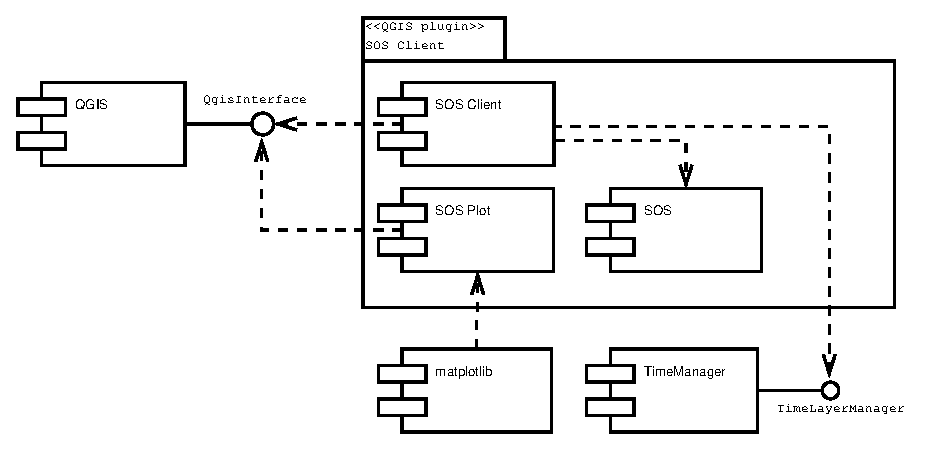
\includegraphics[width=0.5\textwidth]{images/componentes.eps}
 \caption{Diagrama de compoñentes}
 \label{fig:diaComponentes}
\end{figure}

A compoñente \textbf{SOS Client} é a responsable da comunicación co servidor SOS tanto á hora de xerar as peticións necesarias a partir da información proporcionada polo usuario, como para almacenar e interpretar as respostas do servizo.

A compoñente \textbf{SOS Plot} é a responsable de, a partir da capa vectorial xerada, visualizar as observacións segundo as preferencias indicadas polo usuario.

As compoñentes externas incluídas no diagrama son:
\begin{itemize}
\item QGIS: Representa á aplicación na que se integra o \emph{plugin}.
\item TimeManager\footnote{\url{https://plugins.qgis.org/plugins/timemanager/}}: É un \emph{plugin} para QGIS que engade controles de tempo ó mesmo, de xeito que se podan animar as capas vectoriais directamente no visor de mapas, en base a un atributo de tempo.
\item matplotlib\footnote{\url{http://matplotlib.org/}}: É unha librería de Python para debuxar gráficos en 2D que permite producir figuras de alta calidade, tanto para publicacións como en entornos interactivos.
\end{itemize}

\subsection{Patrón de arquitectura}
O uso dun patrón de arquitectura axeitado para o sistema a desenvolver facilita os procesos de implementación e probas, ó proporcionar un esquema de organización estrutural dividindo o sistema en partes segundo a súa responsabilidade.

Os patróns de arquitectura máis amplamente utilizados no desenvolvemento de aplicacións son o MVC (\emph{Model-View-Controller}) e os seus derivados. O obxectivo principal destes patróns é separar o modelo de datos, a súa visualización e a lóxica de negocio facilitando de xeito moi significativo o mantemento e evolución das aplicacións.

Dadas as características concretas desde desenvolvemento optouse por unha simplificación do patrón MVC combinando a lóxica de negocio coas vistas, dando lugar a unha arquitectura denominada \emph{Model/View}\footnote{\url{http://doc.qt.io/qt-4.8/model-view-programming.html}}. Os motivos principais para levar a cabo esta simplificación son:
\begin{itemize}
\item A lóxica de negocio da aplicación e moi sinxela.
\item As librerías para o desenvolvemento das vistas veñen impostas pola aplicación na que se integrará o \emph{plugin}. As propias librerías están deseñadas para facilitar este patrón.
\end{itemize}

É importante destacar que aínda que se se incorpore a lóxica de negocio nas vistas, si que se mantén a separación entre a creación e configuración dos compoñentes gráficos do resto de lóxica da vista. A creación dos compoñentes gráficos faise a través dunha factoría que os xera directamente desde a súa definición XML.

Na figura \ref{fig:MVCvsMV} móstrase de xeito gráfico a diferencia entre o patrón MVC e o \emph{Model/View}. O \emph{Model/View}, amais da vista e o modelo, inclúe o concepto \emph{Delegate}, que representa a un mediador entre a vista e o modelo para facilitar a personalización de como se mostran e editan determinados datos.

\begin{figure}[hbtp]
 \centering
 \includegraphics[width=\textwidth]{images/MVCvsMV.png}
 \caption{Diferencias entre MVC e Model/View}
 \label{fig:MVCvsMV}
\end{figure}

\section{Interacción entre compoñentes}
Para describir o comportamento do sistema desde un punto de vista dinámico empréganse os diagramas de secuencia, nos que se describe a interacción entre as distintas compoñentes do sistema para cumprir cada caso de uso definido.

Para conseguir un nivel de detalle suficiente para describir o comportamento do sistema dividisen as compoñentes segundo a arquitectura \emph{Model/View} proposta. A compoñente SOSClient divídese en SOSClientDialog, que representa a vista, e Sensor Observation Service, que representa o modelo. No caso da compoñente SOSPlot, a vista é representada pola compoñente SOSPlotDialog e o modelo non se representa de xeito independente pois está incluído dentro da compoñente matplotlib.
\newpage
No diagrama \ref{fig:diaSeq1-2} inclúense os caso de uso \ref{uc:CU.01} e \ref{uc:CU.02}, xa que o \ref{uc:CU.02} estende ó \ref{uc:CU.01}, polo que é máis claro representalos xuntos.
\begin{figure}[H]
 \centering
 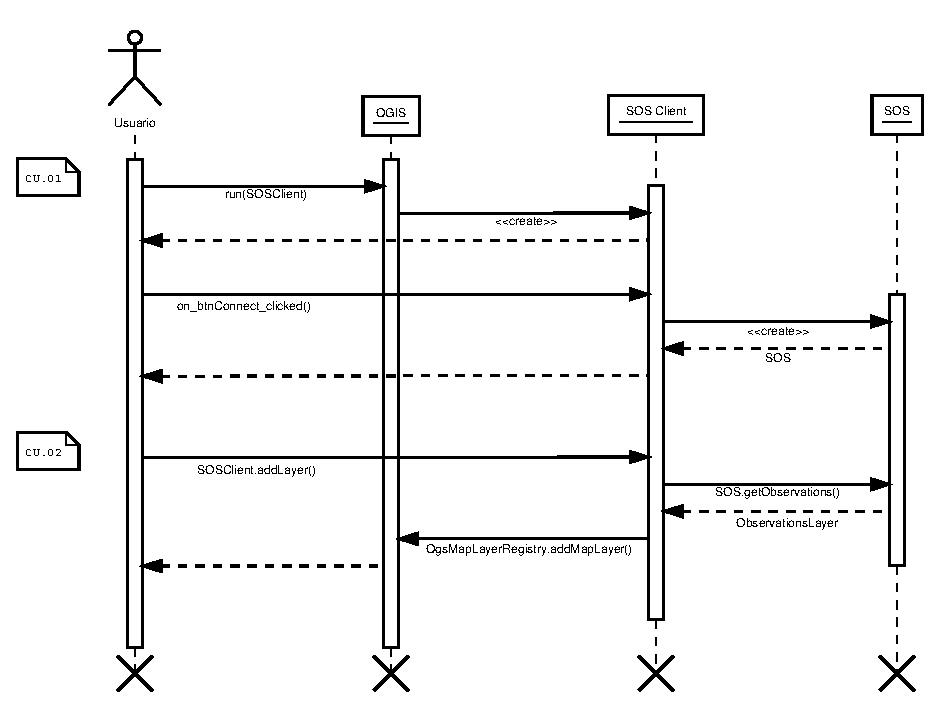
\includegraphics[width=.9\textwidth]{images/seq1-2.eps}
 \caption{Diagrama de secuencia para os casos de uso \ref{uc:CU.01} e \ref{uc:CU.02}}
 \label{fig:diaSeq1-2}
\end{figure}

O diagrama \ref{fig:diaSeq3} representa o comportamento para o caso de uso \ref{uc:CU.03}.
\begin{figure}[H]
 \centering
 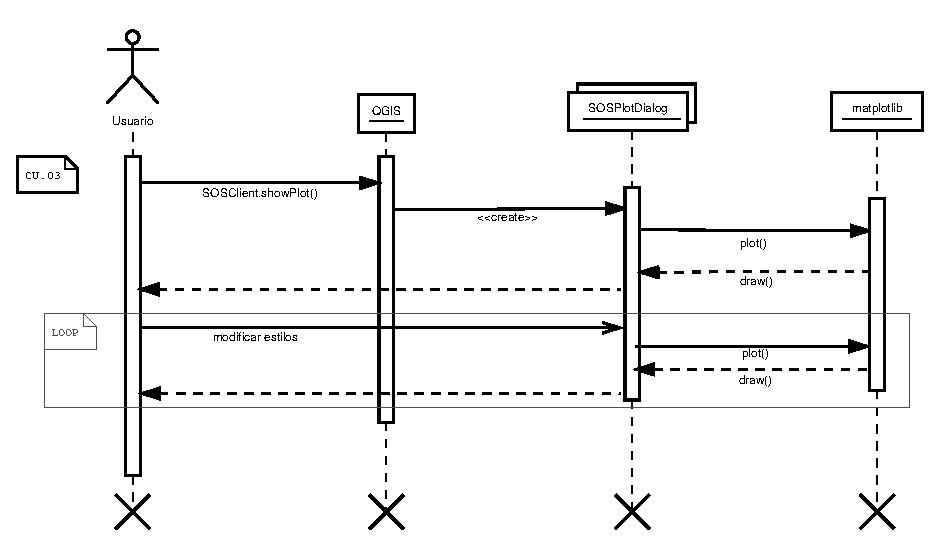
\includegraphics[width=.9\textwidth]{images/seq3.eps}
 \caption{Diagrama de secuencia para o caso de uso \ref{uc:CU.03}}
 \label{fig:diaSeq3}
\end{figure}

Para cubrir a funcionalidade requirida polo caso de uso \ref{uc:CU.04} existe o \emph{plugin} \emph{TimeManager} para QGIS, polo que o que representa o diagrama \ref{fig:diaSeq4} é o procedemento para que a capa xerada coas observacións sexa controlada polo \emph{TimeManager}.
\begin{figure}[H]
 \centering
 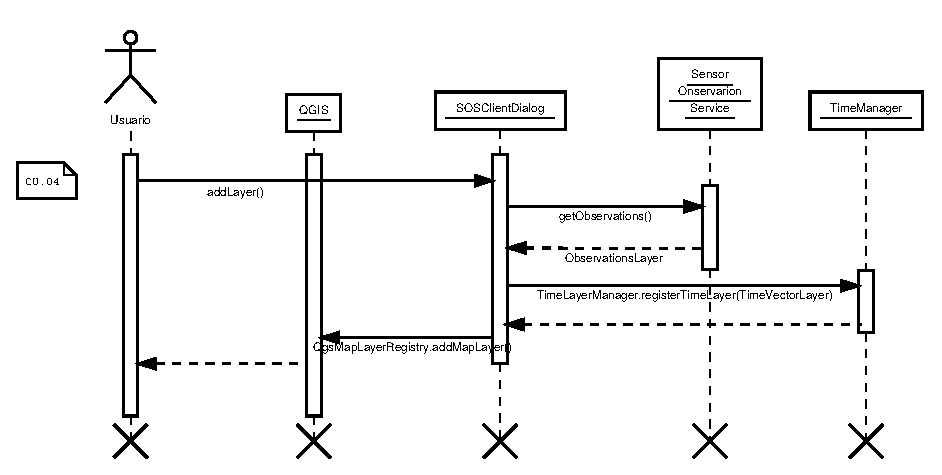
\includegraphics[width=.9\textwidth]{images/seq4.eps}
 \caption{Diagrama de secuencia para o caso de uso \ref{uc:CU.04}}
 \label{fig:diaSeq4}
\end{figure}\cleardoublepage
\chapter{Implementación e probas}
TODO\cleardoublepage
\chapter{Conclusións e traballo futuro}
TODO-Conclusións e posibles ampliacións-
\cleardoublepage

% Aquí empezan os apéndices
\appendix
\chapter{Manual técnico}
\section{Entorno de desenvolvemento}
Se ben non é necesario o uso de ningún entorno de desenvolvemento integrado (IDE) para a modificación do código do plugin, si é recomendable para aumentar a produtividade gracias as funcionalidades como o resaltado de sintaxe, o autocompletado ou a validación automática do código.

A continuación descríbense os pasos a seguir para a instalación dun entorno de desenvolvemento integrado igual ó empregado para a realización do plugin, que se levou a cabo sobre o sistema operativo Ubuntu.

O IDE recomendado na propia documentación de QGIS para o desenvolvemento de plugins en Python é Eclipse\footnote{\url{https://eclipse.org/}} co plugin PyDev\footnote{\url{http://pydev.org/}}, que pode instalarse dende o propio Eclipse. Amais do plugin PyDev tamén debemos instalar o plugin EGit para descargar o código dende GitHub. Tamén debemos ter instalado no equipo o QGIS, que se pode instalar desde os propios repositorios de Ubuntu, o igual que o Eclipse.

Para crear un proxecto desde o repositorio de GitHub existen varias opcións, a máis sinxela sería a seguinte:
\newpage
\begin{itemize}
\item Seleccionar a opción de Import no menú File, e posteriormente Projects from Git.
\begin{figure}[H]
\centering
\includegraphics[width=0.8\textwidth]{images/manualtecnico/import_project01.png}
\caption{Importación do repositorio en Eclipse, paso 1}
\label{fig:import_project01}
\end{figure}
\item Seleccionar a opción GitHub e buscar o repositorio SOS Client.
\begin{figure}[H]
\centering
\includegraphics[width=0.8\textwidth]{images/manualtecnico/import_project02.png}
\caption{Importación do repositorio en Eclipse, paso 2}
\label{fig:import_project02}
\end{figure}
\item Engadir a rama master e importar coa opción Import as general project.
\begin{figure}[H]
\centering
\includegraphics[width=0.8\textwidth]{images/manualtecnico/import_project03.png}
\caption{Importación do repositorio en Eclipse, paso 3}
\label{fig:import_project03}
\end{figure}
\item Unha vez feito importado o proxecto pódese converter nun proxecto de PyDev.
\begin{figure}[H]
\centering
\includegraphics[width=0.8\textwidth]{images/manualtecnico/import_project04.png}
\caption{Importación do repositorio en Eclipse, paso 4}
\label{fig:import_project04}
\end{figure}
\end{itemize}

A continuación débese configurar o PyDev para que recoñeza a API de QGIS e de PyQt4 de forma que teñamos dispoñibles as funcións de autocompletado. Para esto, dende a ventá de Window $\to$ Preferences accedese á configuración do interprete de Python, onde haberá que engadir na lapela de librerías a carpeta $\sim$/.qgis/python/plugins/, e na lapela Forced builtin engadir qgis e PyQt4.
\begin{figure}[H]
\centering
\includegraphics[width=0.75\textwidth]{images/manualtecnico/python_settings.png}
\caption{Configuración de Python en Eclipse}
\label{fig:python_settings}
\end{figure}

Tamén se deben engadir as carpetas do proxecto ó PYTHONPATH, desde as propiedades do proxecto:
\begin{figure}[H]
\centering
\includegraphics[width=0.75\textwidth]{images/manualtecnico/python_path.png}
\caption{Configuración do PYTHONPATH}
\label{fig:python_path}
\end{figure}


O proxecto foi creado inicialmente co plugin 'Plugin Builder'\footnote{\url{http://g-sherman.github.io/Qgis-Plugin-Builder/}} de QGIS polo que contén un Makefile que nos permite usar make coas seguintes opcións, entre outras:
\begin{description}
\item[deploy:] Desprega o plugin na carpeta correspondente.
\item[derase:] Elimina a carpeta de despregue do plugin.
\item[transup:] Actualiza os ficheiros de traducións.
\item[zip:] Desprega o plugin e crea un zip axeitado para subir ó repositorio de QGIS.
\item[test:] Executa os tests.
\end{description}

Tamén é de moita utilidade instalar no QGIS o plugin 'Plugin Reloader'\footnote{\url{http://plugins.qgis.org/plugins/plugin_reloader/}}, que se pode instalar dende o propio menú do QGIS. Este plugin permite volver a cargar un plugin dende disco sen necesidade de cerrar e volver a abrir o QGIS.

Outras ferramentas que se poden necesitar para o desenvolvemento do plugin son o QtDesigner, para modificar os ficheiros de extensión .ui nos que se define a interface gráfica, e o QtLingüist, para as traducións a distintos idiomas.

\section{Ampliación do módulo de procesamento XML}
Co obxectivo de que o módulo de procesamento se poda ampliar para dar cobertura a máis implementacións do servizo SOS e do estándar O\&M este foi deseñado de forma modular, con distintas clases específicas para o procesamento de cada parte do XML. Para engadir soporte para etiquetas xml non soportadas será necesario crear unha clase que herde de XMLParser co nome da etiqueta que procesa co sufixo Parser, de xeito que poda ser instanciada a través da factoría XMLParserFactory cando sexa necesaria.

A clase XMLParser descríbese na figura \ref{fig:xmlparser}, e forma parte do módulo xmlparser no paquete sos.

\begin{figure}[H]
\centering
\begin{minted}[framesep=2mm,bgcolor=gray!20,fontsize=\footnotesize]{python}
class XMLParser (object):
    """
    XML parser base class
    """
    __metadata__ = abc.ABCMeta

    @abc.abstractmethod
    def parse (self, xml=None):
        """
        :param xml: XML to parse
        :type xml: QDomElement or str
        """
    
    @staticmethod
    def searchFirst (xml, query):
        """
        :param xml: XML to parse
        :type xml: QDomNode
        :param query: 
        :type query: str
        :return: QDomNode, str
        """

    @staticmethod
    def search (xml, query):
        """
        :param xml: XML to parse
        :type xml: QDomNode
        :param query: 
        :type query: str
        :return: (QDomNode, str) generator
        """
\end{minted}
\caption{Definición da clase XMLParser}
\label{fig:xmlparser} 
\end{figure}

Esta clase consta de tres métodos. O método \emph{parse} é o que debe ser sobreescrito polas clases fillas, para levar a cabo as operacións que corresponda, e os métodos \emph{searchFirst} e \emph{search} están definidos para abstraer o procesamento do XML das librerías empregadas. Ambas funcións reciben como parámetro o xml sobre o que traballar e a consulta a executar, coa diferencia de que a primeira devolve a primeira ocorrencia, e a segunda permite iterar sobre todas as ocorrencias. O parámetro query permite interrogar por etiquetas, atributos, e atributos con un valor concreto. Por exemplo:

%Configuración para codigo de Python inline
\definecolor{Code}{rgb}{0,0,0}
\definecolor{Decorators}{rgb}{0.5,0.5,0.5}
\definecolor{Numbers}{rgb}{0.5,0,0}
\definecolor{MatchingBrackets}{rgb}{0.25,0.5,0.5}
\definecolor{Keywords}{rgb}{0,0,1}
\definecolor{self}{rgb}{0,0,0}
\definecolor{Strings}{rgb}{0,0.63,0}
\definecolor{Comments}{rgb}{0,0.63,1}
\definecolor{Backquotes}{rgb}{0,0,0}
\definecolor{Classname}{rgb}{0,0,0}
\definecolor{FunctionName}{rgb}{0,0,0}
\definecolor{Operators}{rgb}{0,0,0}
\definecolor{Background}{rgb}{0.98,0.98,0.98}
\lstset{
showspaces=false,
showtabs=false,
showstringspaces=false,
frame=l,
tabsize=4,
% Basic
basicstyle=\ttfamily\small,
backgroundcolor=\color{Background},
language=Python,
% Comments
commentstyle=\color{Comments}\slshape,
% Strings
stringstyle=\color{Strings},
morecomment=[s][\color{Strings}]{"""}{"""},
morecomment=[s][\color{Strings}]{'''}{'''},
% keywords
morekeywords={import,from,class,def,for,while,if,is,in,elif,else,not,and,or,print,break,continue,return,True,False,None,access,as,,del,except,exec,finally,global,import,lambda,pass,print,raise,try,assert},
keywordstyle={\color{Keywords}\bfseries},
% additional keywords
morekeywords={[2]@invariant},
keywordstyle={[2]\color{Decorators}\slshape},
emph={self},
emphstyle={\color{self}\slshape},
}
%Fin de configuración para código Python inline
\begin{itemize}
\item \lstinline|node, version = self.searchFirst (xml, "@version")|\\Devolve o atributo version da etiqueta en curso.
\item \lstinline|for _, value in self.search (xml, "resultModel"): pass|\\Itera sobre todas as etiquetas resultModel fillas do nodo xml.
\item \lstinline|for _, value in self.search (xml, "observedProperty@href"): pass|\\Itera sobre o atributo href de todas as etiquetas observedProperty fillas do nodo xml.
\item \lstinline|for node, tag in self.search (member, "Observation/*"): pass|\\Itera sobre todas as etiquetas fillas de todas as etiquetas Observation fillas do nodo xml.
\item \lstinline|opNode, _ = self.searchFirst (xml, "Operation@name=GetCapabilities")|\\Devolve o primeiro nodo de etiqueta Operation cuxo atributo name vale GetCapabilites.
\end{itemize}

\cleardoublepage
\chapter{Manual de usuario}
\section{Instalación}
TODO: A espera de se o aproban no repositorio oficial, se non o aproban poñer o repositorio a añadir.

O plugin pode instalarse desde a opción 'Administrar e instalar plugins' no menú Plugins do QGIS.
\begin{figure}[hbtp]
\centering
\includegraphics[width=0.8\textwidth]{images/manual/instalar.png}
\caption{Pantalla de instalación do plugin}
\label{fig:install}
\end{figure}

Unha vez instalado engadirase unha nova entrada no menú Web e tres novas accións na barra de ferramentas:
\begin{figure}[hbtp]
\centering
\includegraphics[width=0.8\textwidth]{images/manual/toolbar.png}
\caption{Barra de ferramentas do plugin}
\label{fig:toolbar}
\end{figure}

\begin{description}
\item [{\includegraphics[width=24px]{images/manual/icon_add.png}}] Mostra o diálogo para conectar con un servidor SOS e engadir unha capa de observacións. 
\item [{\includegraphics[width=24px]{images/manual/icon_xml.png}}] Visualiza o ficheiro XML usado para xerar a capa activa. 
\item [{\includegraphics[width=24px]{images/manual/icon_plot.png}}] Xera unha gráfica coas observacións correspondentes ás entidades seleccionadas na capa activa.
\end{description}

\section{Crear capa de observacións}
Ó pulsar a acción \includegraphics[width=16px]{images/manual/icon_add.png} mostrarase o formulario da figura TODO. Neste formulario pódese xestionar a lista de servidores cos botóns Novo, Editar e Eliminar, e co botón Conectar visualizar as capacidades do servidor seleccionado.
\begin{figure}[hbtp]
\centering
\includegraphics[width=\textwidth]{images/manual/tabInfo-limpia.png}
\caption{Diálogo de conexión co servidor, sen datos}
\label{fig:tabInfo-limpia}
\end{figure}

Unha vez se conectou con un servidor móstranse as súas capacidades na lapela Información (figura \ref{fig:tabInfo}).
\begin{figure}[hbtp]
\centering
\includegraphics[width=\textwidth]{images/manual/tabInfo.png}
\caption{Diálogo de conexión co servidor, con datos}
\label{fig:tabInfo}
\end{figure}

Para obter as observacións débese seleccionar unha oferta no campo Ofertas e pódese modificar no Nome da capa. As distintas lapelas do formulario descríbense no cadro \ref{tab:lapelas}:
\begin{table}	
\begin{tabularx}{\textwidth}{cX}
	\raisebox{-0.8\totalheight}{\includegraphics[width=0.4\textwidth]{images/manual/tabPropiedades.png}} & 
	Lista de propiedades da oferta. Pode seleccionar unha ou varias.\\
	\\
	\raisebox{-0.8\totalheight}{\includegraphics[width=0.4\textwidth]{images/manual/tabEntidades.png}} & Lista de entidades da oferta. Pode seleccionar varias ou ningunha.\\
	\\
	\raisebox{-0.8\totalheight}{\includegraphics[width=0.4\textwidth]{images/manual/tabProcedementos.png}} & Lista de procedementos. Pode seleccionar varios ou ningún.\\
	\\
	\raisebox{-0.8\totalheight}{\includegraphics[width=0.4\textwidth]{images/manual/tabFiltros.png}} & Filtros dispoñibles. Pódense activar varios ó mesmo tempo. No caso do espacial, pulsando na icona poderase seleccionar a xeometría a consultar debuxando no mapa como se amosa na figura \ref{fig:spatialtool}.\\
	\\
	\raisebox{-0.8\totalheight}{\includegraphics[width=0.4\textwidth]{images/manual/tabResultado.png}} & Pódese seleccionar o modelo de resultado entre os dispoñibles para o servidor. Permite indicar se todas as entidades terán información xeométrica ou so a primeira para cada \emph{foi} e seleccionar se engadir a capa ó TimeManager. Tamén se pode seleccionar o directorio de traballo no que se gardan os datos descargados.\\
\end{tabularx}
\caption{Lapelas do formulario de consulta ó SOS}
\label{tab:lapelas}
\end{table}

\begin{figure}[hbtp]
\centering
\includegraphics[width=\textwidth]{images/manual/spatialtool.png}
\caption{Ferramenta de selección espacial}
\label{fig:spatialtool}
\end{figure}

Unha vez seleccionadas as opcións desexadas pódese engadir a capa ó QGIS pulsando no botón Engadir, ou cambiar o XML a enviar antes de engadir a capa co botón 'Editar petición', como se ve na figura \ref{fig:editarPeticion}.

\begin{figure}[hbtp]
\centering
\includegraphics[width=\textwidth]{images/manual/editar_peticion.png}
\caption{Engadir capa SOS}
\label{fig:editarPeticion}
\end{figure}

\section{Gráficos en dúas dimensións}

Para visualizar un gráfico é necesario que a capa activa teña unha ou máis entidades seleccionadas, e despois premer no botón \includegraphics[width=16px]{images/manual/icon_plot.png}, como se amosa na figura \ref{fig:ejecutarSOSPlot}.

\begin{figure}[hbtp]
\centering
\includegraphics[width=\textwidth]{images/manual/ejecutar_sosplot.png}
\caption{Executar ferramenta SOS Plot}
\label{fig:ejecutarSOSPlot}
\end{figure}

Esta operación abrirá unha nova ventá (figura \ref{fig:sosplot}) na que se visualizará a gráfica, e na que se poden editar as opcións do mesmo e interactuar coa gráfica.

\begin{figure}[hbtp]
\centering
\includegraphics[width=\textwidth]{images/manual/sosplot.png}
\caption{SOS Plot: Gráfica de varias series}
\label{fig:sosplot}
\end{figure}

Neste formulario pódese editar o título do gráfico e dos eixos, a propiedade a representar en cada eixo e os límites dos mesmos, o formato no que representar o tempo, a inclusión dunha lenda, e o estilo e cor de liña e marcador de cada unha das series debuxadas. Amais sobre a gráfica pódese facer zoom, desprazala e gardar a imaxe.\cleardoublepage

\nocite{*}
\bibliography{bibliografia}
\bibliographystyle{plain}
\end{document}
